\chapter{Portfolio Diversification and Supporting Financial Institutions}

In Robert J. Shiller's fourth lecture on financial markets, as curated by LazyingArt LLC, the mathematics is deliberately delayed. We begin with a historical invention, not with an optimization problem. The VOC, the Amsterdam Stock Exchange, brokers, street-name ownership, short selling, and limited liability all appear before any frontier is drawn. Only after that world is in place do we ask the lecture's central quantitative question: if expected returns, variances, and covariances are given, how should we think about a portfolio? The answer unfolds step by step: first leverage, then hyperbolas, then diversification, then tangency, and finally the CAPM intuition that the risk which matters is covariance with the market.

\section{Finance as Institutional Invention}

The lecture opens by returning to the previous lecture's theme that finance is a branch of engineering. Financial arrangements are invented to perform functions; when they work, they spread. That is the spirit in which the lecture turns to 1602 and to the Verenigde Oostindische Compagnie, together with the Amsterdam Stock Exchange built to trade its shares.

\begin{definition}
A portfolio is a collection of investments held over a specified horizon.
\end{definition}

This historical prelude matters because the lecture does not want to treat portfolio theory as a detached theorem. The VOC was not a one-voyage merchant partnership that dissolved when the ships came home. It was a long-term company, meant to continue indefinitely, to build trading posts across the world, and to attract capital from a broad public. Once such a company exists, the lecture argues, a whole institutional framework begins to arise almost automatically.

Shares become tradable every day rather than only when the company reopens its books. Brokers hold inventories and intermediate between buyers and sellers. Ownership is effectively held in what we would now call street name: the broker's records tell the investor that he owns the shares, even before the company itself updates its own books. And once that arrangement exists, a broker can sell more shares than he currently owns and plan to acquire them later. Short interest is not an exotic later invention. It appears naturally once the market is liquid enough.

The lecture lingers over this point because it is one of the main institutional morals. A large, durable, tradable company does not produce calm. It produces disagreement, speculation, and volatility. Some traders become wildly optimistic and bid the stock up; others become pessimistic and short it. The market becomes active because the value is uncertain, and the value is felt to be uncertain because the market is active.

The same is true of limited liability. If shareholders can lose no more than the funds they invest, then a much wider public can take part in risky enterprise. One need not inspect every ship captain or every distant trading post personally. One can buy the stock and know that the downside is capped at the original investment. In that sense the stock market is a social technology. It channels appetite for risk into the financing of large productive ventures.

This is why the opening history is not decorative. The lecture is showing us the institutional soil out of which portfolio theory grows. Once tradable risky claims exist and once they fluctuate in public view, the question of how to hold them becomes unavoidable.

\section{The Equity Premium Puzzle}

From that institutional prelude the lecture pivots into a puzzle. One can already hear it in the VOC story. Suppose an equity claim appears to earn astonishing returns year after year. Why does capital not flood into it until the extraordinary advantage disappears?

The lecture broadens that question beyond the VOC itself. The striking point is not merely that one famous stock once did well. The point is that common stocks seem to have done very well over very long periods. In the U.S. data cited in the lecture, the real geometric average return on stocks is about \(6.8\%\) per year, whereas the real return on short-term government securities is only about \(2.8\%\). The difference is therefore about
\begin{equation}
6.8\% - 2.8\% = 4.0\%.
\end{equation}
That is already a large gap. The lecture then adds that in the long U.S. sample under discussion there was no rolling thirty-year period in which stocks underperformed safe short-term government claims or long-term bonds.

The same broad phenomenon appears internationally. The lecture cites evidence from Dimson, Marsh, and Staunton: across the countries they study, stocks outperform bonds, with equity premia running from about \(3\%\) to about \(6\%\). The puzzle is therefore not parochial. It is not just a peculiarity of the United States.

This is where the lecture deliberately slows down. If equities have performed so well for so long, why does everyone not simply learn the lesson and hold them?

\subsection{Question \& Answer}

\paragraph{Question.} If stocks do so well, why does everyone not simply hold them?

\paragraph{Answer.} The lecture's first answer is the standard one: risk. Stocks are riskier; the extra return is a risk premium. But the lecture does not allow that answer to stand in vague form. What exactly is the relevant risk? Is it just price fluctuation taken by itself? Or is the matter subtler once assets are placed inside a portfolio? That is the point of transition. The lecture is not satisfied with the slogan that stocks are volatile. It wants a theory of why that volatility matters and of how portfolio structure changes the answer.

At this point the lecture introduces Harry Markowitz. The move is methodological. Before 1952, investors knew the proverb about not putting all their eggs in one basket. But the lecture insists that this was not yet a theory. It was good advice without a mathematical problem attached to it. Markowitz changed the subject by asking: if we know expected returns, variances, and covariances, what portfolio should we choose?

\section{Markowitz's Breakthrough and the One-Risky-One-Riskless Case}

The lecture treats Markowitz's 1952 paper as a genuine conceptual break. In retrospect the problem sounds obvious. But that is part of the point: it sounded obvious only after someone finally asked it sharply. What had existed before was a loose culture of investing and advice literature. What Markowitz supplied was a well-posed problem in which the inputs are expected returns, variances, and covariances, and the output is a portfolio choice.

The lecture dramatizes this by imagining a mathematically inclined portfolio manager. We are given a one-year horizon. We gather historical data on every possible investment we can think of. We compute average returns, variances, covariances, and correlations. Then we step back from judgment and prediction and ask the stripped-down mathematical question: if these statistics are taken as given, what is the best portfolio? The lecture's astonishment is that such a question was not standard long before 1952.

A small historical aside reinforces the point. The lecture notes that older investment manuals did say ``do not put all your eggs in one basket.'' But they stopped there. They did not say how to diversify, how much to hold, or why a particular mix is optimal. That is exactly the gap Markowitz filled.

The lecture begins the formal analysis with the simplest nontrivial case: one risky asset and one riskless asset. The risky asset may first be imagined as the VOC itself. The riskless asset may be taken, approximately, to be a short government claim whose maturity matches the investor's horizon.

\subsection{Question \& Answer}

\paragraph{Question.} If leverage lets us reach many target returns from one risky asset, what could an ``optimal portfolio'' even mean?

\paragraph{Answer.} It cannot mean ``the best asset'' in isolation. Once borrowing, lending, and shorting are allowed, a single risky asset already generates a whole menu of feasible portfolios. So the right question is not ``What is the best investment?'' but rather ``What tradeoff between expected return and risk do we want?'' That is the first genuinely Markowitzian turn in the lecture.

\begin{figure}[h]
\centering

\includegraphics[width=0.82\textwidth]{lecture_04_figure_02.png}
\caption{Lecture slide: risky and riskless asset portfolio formulas.}
\end{figure}

The slide visible at this point in the lecture is worth keeping because its order of presentation is itself instructive: first the allocation, then expected return, then variance, then standard deviation, and only then the reduced relation between standard deviation and expected return. The slide says ``portfolio expected value,'' but the lecture is plainly using expected return. We standardize the notation while preserving the lecture's sequence.

If a fraction \(x\) of wealth is placed in the risky asset and \(1-x\) in the riskless asset, then
\begin{align}
r_p &= x r_1 + (1-x)r_f, \\
\operatorname{Var}(r_p) &= x^2 \operatorname{Var}(r_1), \\
\sigma_p &= |x| \sigma_1.
\end{align}
The variance expression is simple because the riskless return is known at the horizon. The lecture then solves the expected-return equation for \(x\):
\begin{equation}
x = \frac{r_p-r_f}{r_1-r_f}.
\end{equation}
Substituting this into the expression for standard deviation gives the cleaned version of the bottom slide formula:
\begin{equation}
\sigma_p
=
\left|
\frac{r_p-r_f}{r_1-r_f}
\right|
\sigma_1.
\end{equation}
This is the lecture's reduced formula for the broken straight line in \((\sigma_p,r_p)\)-space.

\paragraph{Worked example.}
The lecture's numerical example chooses a riskless rate of \(5\%\), a risky-asset expected return of \(20\%\), and a risky-asset standard deviation of \(40\%\). It begins not with an abstract weight \(x\), but with guilders.

\begin{enumerate}
\item Suppose we have \(100\) guilders and put them all into the risky asset. Then the expected profit is \(20\) guilders and the standard deviation is \(40\) guilders.
\item Suppose instead we borrow another \(100\) guilders and invest \(200\) guilders in the risky asset. Then the asset side has expected gain \(40\) guilders, but the loan costs \(5\) guilders in interest. So the expected return on our original wealth is
\begin{equation}
2(20\%) - 5\% = 35\%.
\end{equation}
The standard deviation doubles with the position size:
\begin{equation}
2(40\%) = 80\%.
\end{equation}
\item Now go the other way and short \(200\) guilders of the risky asset. The short position has expected loss \(40\) guilders, while the \(300\) guilders held in cash earn \(5\%\), or \(15\) guilders. So the expected return on the original wealth is
\begin{equation}
-2(20\%) + 3(5\%) = -25\%.
\end{equation}
\end{enumerate}

The lecture then turns the bookkeeping into geometry. If we plot standard deviation on the horizontal axis and expected return on the vertical axis, the feasible set becomes a broken straight line issuing from the riskless point: an upward branch for lending and leveraged long positions, and a downward branch for sufficiently large short positions. The lecture explicitly calls this a degenerate hyperbola.

\begin{figure}[h]
\centering
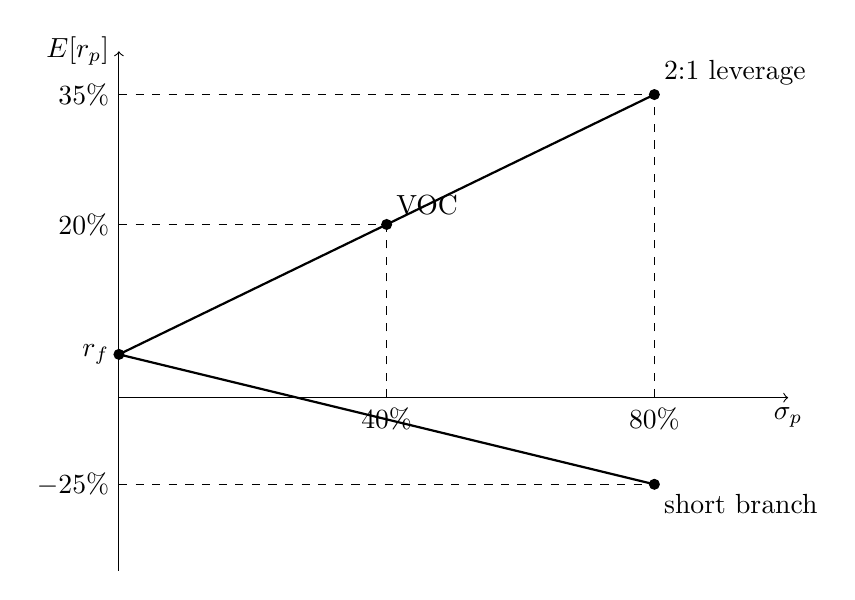
\begin{tikzpicture}[x=0.85cm,y=0.55cm]
\draw[->] (0,0) -- (10,0) node[below] {$\sigma_p$};
\draw[->] (0,-4) -- (0,8) node[left] {$E[r_p]$};

\draw[thick] (0,1) -- (8,7);
\draw[thick] (0,1) -- (8,-2);

\fill (0,1) circle (2pt);
\fill (4,4) circle (2pt);
\fill (8,7) circle (2pt);
\fill (8,-2) circle (2pt);

\draw[dashed] (4,0) -- (4,4);
\draw[dashed] (0,4) -- (4,4);
\draw[dashed] (8,0) -- (8,7);
\draw[dashed] (0,7) -- (8,7);
\draw[dashed] (0,-2) -- (8,-2);

\node[left] at (0,1) {$r_f$};
\node[above right] at (4,4) {VOC};
\node[above right] at (8,7) {2:1 leverage};
\node[below right] at (8,-2) {short branch};
\node[below] at (4,0) {$40\%$};
\node[below] at (8,0) {$80\%$};
\node[left] at (0,4) {$20\%$};
\node[left] at (0,7) {$35\%$};
\node[left] at (0,-2) {$-25\%$};
\end{tikzpicture}
\caption{Transcript-based reconstruction of the one-risky-one-riskless opportunity set.}
\end{figure}

This is where the lecture makes its first big philosophical move. If a client asks for \(100\%\) expected return, one can produce it by leverage. That does not make the portfolio manager a genius. It only means that the menu is already wide. There is no single best investment here, only a tradeoff between return and standard deviation. That is why the lecture says that before we have multiple risky assets, we have not yet fully gotten into Markowitz.

\section{Two Risky Assets and the Efficient Frontier}

Now the lecture leaves the degenerate case behind and moves to the first true Markowitz curve. We temporarily set the riskless asset aside and imagine two risky assets. In the numerical example used in the lecture, these are U.S. stocks and long-term Treasury bonds held over a one-year horizon. The latter are called ``bonds,'' but the lecture is careful to say that they are not riskless here, because their market price changes over the year.

\begin{figure}[h]
\centering

\includegraphics[width=0.82\textwidth]{lecture_04_figure_03.png}
\caption{Lecture slide: two-asset frontier variance substitution.}
\end{figure}

If \(x_1\) is the weight in asset \(1\) and \(1-x_1\) is the weight in asset \(2\), then the portfolio expected return is
\begin{equation}
r_p = x_1 r_1 + (1-x_1)r_2.
\end{equation}
The lecture then repeats the same logical move as before: solve for the weight in terms of the target return. The slide shows
\begin{equation}
x_1 = \frac{r_p-r_2}{r_1-r_2}.
\end{equation}
The underlying two-asset portfolio variance formula, standard in this setting, is
\begin{equation}
\sigma_p^2 = x_1^2 \sigma_1^2 + (1-x_1)^2 \sigma_2^2 + 2x_1(1-x_1)\sigma_{12}.
\end{equation}
Substituting the solved expression for \(x_1\) produces the visible frontier formula:
\begin{align}
\sigma_p^2
&=
\left(
\frac{r_p-r_2}{r_1-r_2}
\right)^2
\sigma_1^2
+
\left(
\frac{r_1-r_p}{r_1-r_2}
\right)^2
\sigma_2^2
+
2
\frac{(r_p-r_2)(r_1-r_p)}{(r_1-r_2)^2}
\sigma_{12}.
\end{align}

This is the lecture's first genuine hyperbola. The covariance term is not an afterthought. It is the reason the curve bends inward. If the two assets do not move perfectly together, then combining them can reduce risk in a way that no single-asset comparison could have revealed.

\begin{figure}[h]
\centering
\begin{tikzpicture}[x=0.48cm,y=0.55cm]
\draw[->] (0,0) -- (22,0) node[below] {$\sigma_p$};
\draw[->] (0,0) -- (0,10) node[left] {$E[r_p]$};

\draw[thick] plot[smooth] coordinates {(7.0,5.4) (8.0,6.1) (10.0,6.9) (13.5,7.9) (18.0,8.8)};
\draw[thick,dashed] plot[smooth] coordinates {(7.0,5.4) (7.8,4.8) (9.5,4.0) (12.5,2.6)};

\fill (9.5,4.0) circle (2pt);
\fill (8.2,5.8) circle (2pt);
\fill (10.2,6.6) circle (2pt);
\fill (16.0,8.3) circle (2pt);

\node[below] at (9.5,4.0) {100\% bonds};
\node[left] at (8.2,5.8) {$25/75$};
\node[above] at (10.2,6.6) {$50/50$};
\node[right] at (16.0,8.3) {100\% stocks};

\draw[dotted] (7.0,0) -- (7.0,5.4);
\node[below] at (7.0,0) {$\sigma_{\min}$};
\node[above right] at (13.2,7.8) {efficient frontier};
\end{tikzpicture}
\caption{Simplified redraw of the two-asset opportunity set. The efficient frontier is the upper branch above the minimum-variance point.}
\end{figure}

The lecture now asks, in its own voice, ``What do we learn from this?'' The first answer is that the whole curve is not efficient. Only the upper branch above the minimum-variance point belongs to the efficient frontier. The second answer is much sharper: a \(100\%\) bond portfolio is dominated. There exists a stock-bond mixture with the same standard deviation and a higher expected return.

This is one of the lecture's most memorable practical claims. A conservative portfolio is not automatically rational just because it carries a familiar label such as ``all bonds.'' Once the geometry is drawn, we can see that some seemingly prudent choices lie strictly below the efficient set. The lecture even remarks that this now looks obvious and yet once was not. That is why it treats Markowitz as such a fundamental breakthrough.

The lecture's fondness for geometry is not ornamental here. It briefly invokes Apollonius and conic sections to make the point that the hyperbola is doing real conceptual work. The curve is teaching us something about investment choice that was not obvious before we drew it.

\section{Three Assets, Diversification, and Oil}

Having gone from one risky asset to two, the lecture now goes one step further and adds oil. The transition is important: the two-asset case gives us the frontier geometry, but the three-asset case gives us the lecture's main application of diversification.

\begin{remark}
At this point the transcript garbles some of the third-asset subscripts. The formulas below are standard reconstructions that match the lecturer's intended meaning and the visible frontier chart. They should be read as careful normalization rather than as a literal transcription of every spoken symbol.
\end{remark}

With three risky assets, expected return remains a weighted average:
\begin{equation}
r_p = x_1 r_1 + x_2 r_2 + x_3 r_3,
\qquad
x_1+x_2+x_3=1.
\end{equation}
The portfolio variance becomes
\begin{align}
\sigma_p^2
&=
x_1^2 \sigma_1^2
+
x_2^2 \sigma_2^2
+
x_3^2 \sigma_3^2
+
2x_1x_2 \sigma_{12}
+
2x_1x_3 \sigma_{13}
+
2x_2x_3 \sigma_{23}.
\end{align}
The lecture's chart should then be read as follows: for each target expected return, solve for the minimum-variance mixture of stocks, bonds, and oil. The resulting set of minimizing portfolios traces a new frontier.

\begin{figure}[h]
\centering

\includegraphics[width=0.88\textwidth]{lecture_04_figure_04.png}
\caption{Lecture slide: efficient frontier with and without oil.}
\end{figure}

The slide is visually dense and worth keeping as evidence. The old stock-bond frontier remains on it as the weaker comparison set, labeled ``W/O Oil.'' The new frontier, labeled ``With Oil,'' lies to the left over the relevant range. That leftward shift is the lecture's main diversification result: once we add an asset that offers return and is not highly correlated with the stock market, we can attain the same expected return with less standard deviation.

The lecture likes to say this in deliberately ordinary language: more eggs in the basket, not fewer. That is the inversion of the old proverb. The point is not to spread wealth thinly at random. The point is that, once covariances enter the picture, more asset classes can make the whole portfolio safer for a given target return.

The visible labels on the slide support the narrative. We can still see benchmark portfolios such as \(100\%\) bonds, \(50\%\) stocks and \(50\%\) bonds, and \(100\%\) stocks. But once oil is available, the frontier includes mixtures such as \(15\%\) oil, \(53\%\) stocks, \(32\%\) bonds, and \(21\%\) oil, \(79\%\) stocks, \(0\%\) bonds. At the upper end one labeled point even uses a negative bond weight, reminding us that the frontier can combine diversification with leverage.

\begin{figure}[h]
\centering
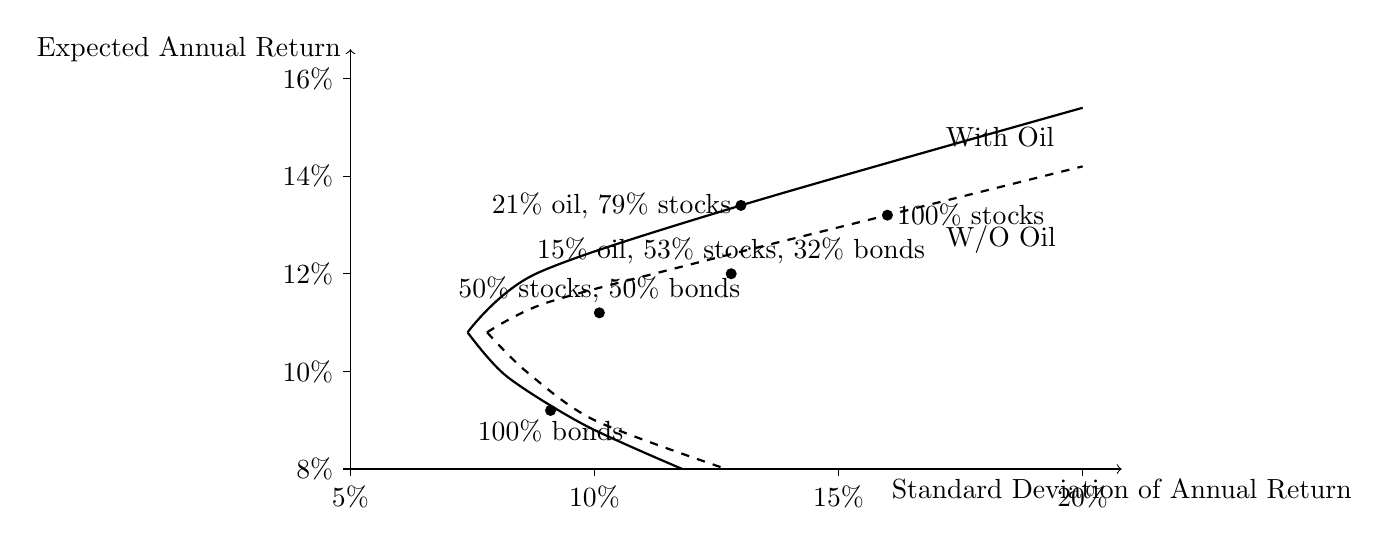
\begin{tikzpicture}[x=0.62cm,y=0.62cm]
\draw[->] (5,8) -- (20.8,8) node[below] {Standard Deviation of Annual Return};
\draw[->] (5,8) -- (5,16.6) node[left] {Expected Annual Return};

\foreach \x in {5,10,15,20}
{
  \draw (\x,8) -- (\x,7.85);
  \node[below] at (\x,7.85) {\(\x\%\)};
}
\foreach \y in {8,10,12,14,16}
{
  \draw (5,\y) -- (4.85,\y);
  \node[left] at (4.85,\y) {\(\y\%\)};
}

\draw[thick,dashed] plot[smooth] coordinates {(7.8,10.8) (9.0,11.4) (12.0,12.2) (16.0,13.2) (20.0,14.2)};
\draw[thick,dashed] plot[smooth] coordinates {(7.8,10.8) (8.6,10.0) (10.0,9.0) (12.7,8.0)};

\draw[thick] plot[smooth] coordinates {(7.4,10.8) (8.8,12.0) (13.0,13.4) (20.0,15.4)};
\draw[thick] plot[smooth] coordinates {(7.4,10.8) (8.2,9.9) (9.8,8.9) (11.8,8.0)};

\fill (9.1,9.2) circle (2pt);
\fill (10.1,11.2) circle (2pt);
\fill (12.8,12.0) circle (2pt);
\fill (16.0,13.2) circle (2pt);
\fill (13.0,13.4) circle (2pt);

\node[below] at (9.1,9.2) {100\% bonds};
\node[above] at (10.1,11.2) {50\% stocks, 50\% bonds};
\node[above] at (12.8,12.0) {\(15\%\) oil, \(53\%\) stocks, \(32\%\) bonds};
\node[right] at (16.0,13.2) {100\% stocks};
\node[left] at (13.0,13.4) {\(21\%\) oil, \(79\%\) stocks};

\node[right] at (17.0,14.8) {With Oil};
\node[right] at (17.0,12.7) {W/O Oil};
\end{tikzpicture}
\caption{Simplified redraw of the frontier comparison, preserving the lecture's truncated horizontal axis beginning at \(5\%\).}
\end{figure}

The lecture then turns back from mathematics to institutions. Norway is described as having far too much implicit oil exposure, not because its statisticians cannot do the arithmetic, but because oil is politically and symbolically charged. The lecturer's argument is that Norway need not literally sell the oil in the ground in order to diversify; it could reduce exposure with derivative transactions, for example by shorting oil futures. Yet politics makes such hedging difficult. Mexico appears as a similar example. The lesson is that correct geometry does not automatically become actual policy.

The lecture also takes care to sharpen the frontier concept once more. If we ask for the minimum-variance portfolio that delivers, say, a \(9\%\) return, we may land at \(100\%\) bonds. But that point is still not efficient if a higher-return point exists at the same standard deviation. So the efficient frontier is only the upper branch above the minimum-variance point. Minimum variance by itself is not the same thing as best.

\begin{figure}[h]
\centering

\includegraphics[width=0.88\textwidth]{lecture_04_figure_05.png}
\caption{Lecture slide: the horizontal axis begins at \(5\%\), not at zero.}
\end{figure}

This second screenshot of the oil chart matters for a different reason. Here the lecturer points directly to the left end of the horizontal axis and remarks that the diagram does not show zero. That observation is not incidental. It prepares the next step. Once we add the riskless asset back into the picture, the relevant line begins at zero standard deviation on the vertical axis at the riskless return. The oil chart is a picture of risky portfolios only; it is not yet the full geometry.

\section{The Riskless Asset Returns: Tangency, Mutual Funds, and Market Risk}

Now the lecture returns to the riskless asset. The move is deliberately parallel to the earlier one-risky-one-riskless example. We take any efficient risky portfolio on the frontier and treat it as a single composite risky asset. Then we ask what happens when we mix that composite with the riskless asset.

Geometrically the answer is simple. Any mixture of a given risky portfolio and the riskless asset lies on a straight line. So the problem becomes: which straight line through the riskless point lies highest? The lecture phrases it in exactly that way. Start from the riskless return on the vertical axis and draw the highest feasible straight line. The portfolio at which that line touches the efficient risky frontier is the tangency portfolio.

If \(r_T\) and \(\sigma_T\) denote the expected return and standard deviation of that tangency portfolio, then every mixture of the riskless asset and that portfolio lies on the capital market line
\begin{equation}
E[r_p] = r_f + \frac{E[r_T]-r_f}{\sigma_T}\,\sigma_p.
\end{equation}
The lecture does not derive this equation algebraically, but it does derive the geometry that the equation expresses.

This restores, in a subtler form, the idea of an optimal portfolio. Earlier the lecture argued that there is no single best investment in the crude sense. With only one risky asset and a riskless asset, we had a whole broken line of possibilities. With many risky assets and no riskless asset, we had a hyperbolic frontier of efficient but taste-dependent choices. But once the riskless asset is available again, a special risky portfolio emerges: the tangency portfolio. Everyone who is efficient wants to lie on the same line and therefore wants to hold the same risky fund, scaled up or down by borrowing or lending.

\begin{proposition}
Under the lecture's Markowitz assumptions---shared expected returns, shared variances and covariances, and the ability to borrow or lend at the riskless rate---every efficient portfolio is a mixture of the riskless asset and the same tangency portfolio.
\end{proposition}

\begin{proof}
Fix any efficient risky portfolio on the frontier. Mixing it with the riskless asset produces a straight line through the riskless point. Among all such lines, only the one with maximal slope delivers the highest expected return for every attainable standard deviation. That maximal-slope line is tangent to the risky frontier. Therefore any efficient investor chooses a point on that same line and differs from any other efficient investor only in the scale of the holding in the riskless asset versus the tangency portfolio.
\end{proof}

This is the mutual fund theorem in the lecture's form. One need not search endlessly among fundamentally different efficient risky funds. Under the theory's assumptions, there is one. Investors differ not in the identity of the risky portfolio, but in how much leverage or de-leverage they want around it.

The lecture then takes the market-clearing step. If all investors want to hold the same risky portfolio, that portfolio must be the aggregate portfolio of risky assets outstanding. Otherwise supply and demand would not match. Hence
\begin{equation}
\text{market portfolio} = \text{tangency portfolio}.
\end{equation}
This is the bridge from Markowitz geometry to equilibrium asset pricing.

The lecture does not give a full derivation of the capital asset pricing model. It states the canonical relation and then interprets it:
\begin{equation}
E[r_i] = r_f + \beta_i\bigl(E[r_M]-r_f\bigr),
\end{equation}
with
\begin{equation}
\beta_i = \frac{\operatorname{Cov}(r_i,r_M)}{\operatorname{Var}(r_M)}.
\end{equation}
The central interpretive point is that investors do not care about standalone variance once an asset can be embedded inside a diversified portfolio. Idiosyncratic fluctuations can be averaged away. What remains costly is covariance with the market, because that risk survives diversification. In the lecture's own language, risk is no longer mere uncertainty. Risk is co-movement with the market.

That is why beta matters. A high-beta stock is not merely a stock with a jumpy price. It is a stock whose return moves strongly with the market's return. The lecture gives Apple, with beta around \(1.5\), as an example of an asset that responds to market movements in an amplified way. That market exposure is what commands extra expected return.

The final practical coda is the Sharpe ratio:
\begin{equation}
S_p = \frac{E[r_p]-r_f}{\sigma_p}.
\end{equation}
Along the tangency line, this ratio is constant. Geometrically it is just the slope of the line from the riskless point to the portfolio. Economically it is a correction for leverage. A manager who advertises a \(15\%\) average return may simply be levering up an ordinary risky strategy. The Sharpe ratio asks instead how much excess return was earned per unit of standard deviation.

This is how the lecture ends: with a theory that begins by redefining risk and closes by telling us how to evaluate portfolio managers. The mathematics is not an ornament. It is a way of refusing to be impressed by raw return without asking what leverage and what market exposure produced it.

\section{Summary}

The lecture begins with institutions and ends with equilibrium asset pricing, and the order is the argument. We first see finance as invention: the VOC, the Amsterdam exchange, brokers, street-name ownership, short interest, limited liability, and volatility. That institutional world then raises the equity premium puzzle. Markowitz enters by turning a proverb about diversification into a mathematical problem stated in terms of expected returns, variances, and covariances. With one risky asset and one riskless asset, we discover that there is no single best investment, only a risk-return tradeoff. With two risky assets, the feasible set becomes a hyperbola and dominated portfolios become visible. With three risky assets, diversification becomes a geometry of leftward shifts in the frontier, even if institutions and politics resist the prescription. Finally, when the riskless asset is added back, the tangency portfolio, the mutual fund theorem, the market portfolio, the CAPM intuition, and the Sharpe ratio all fall into place. The lecture's deeper lesson is that risk is not a property of an asset in isolation. It is a property of the asset inside the portfolio and, in the end, inside the market.